\documentclass[tikz]{beamer}
\usetheme[hideothersubsections]{Hannover}
\usepackage{fontspec}
\usepackage{stmaryrd,amsthm,amsmath,amssymb}
\usepackage{unicode-math}
\usepackage{color,graphicx,subfig}
\usepackage{tikz,pgfplots}
\usepackage{aircraftshapes}
\usepackage{algorithm,algpseudocode}
\usepackage{tabulary}

\usetikzlibrary{intersections}
\usetikzlibrary{decorations.pathmorphing}

\usecolortheme{dolphin}

\title[Reconfiguration par Monte Carlo]{%
  Recherche arborescente Monte Carlo applique au probleme de reconfiguration
  dynamique de l'espace aerien
}
\author[Hondet, Viry]{G.~Hondet, B.~Viry}

% ----------------------------------------------------------
% nuremotation des pages -----------------------------------
% ----------------------------------------------------------
\def\swidth{1.6cm}
\setbeamersize{sidebar width left=\swidth}
\setbeamertemplate{sidebar left}
{%
  {\usebeamerfont{title in sidebar}
    \vskip1.5em
    \usebeamercolor[fg]{title in sidebar}
    \insertshorttitle[width=\swidth,center,respectlinebreaks]\par
    \vskip1.25em
  }
  {
    \usebeamercolor[fg]{author in sidebar}
    \usebeamerfont{author in sidebar}
    \insertshortauthor[width=\swidth,center,respectlinebreaks]\par
    \vskip1.25em
  }
  \hbox to2cm{\hss\insertlogo\hss}
  \vskip1.25em
  \insertverticalnavigation{\swidth}
  \vfill
  \hbox to2cm{\hskip0.6cm\usebeamerfont{subsection in
      sidebar}\strut\usebeamercolor[fg]{subsection in
      sidebar}\insertframenumber /\inserttotalframenumber\hfill}
  \vskip3pt
}
% ----------------------------------------------------------

\begin{document}
\begin{frame}
  \titlepage{}
\end{frame}

\AtBeginSection[]
{%
  \begin{frame}
    \frametitle{Plan}
    \tableofcontents[currentsection]
  \end{frame}
}

\section*{Introduction}

\begin{frame}[c]{Introduction}
  \begin{itemize}
    \item But: diminution de la charge de travail des controleurs
    \item Actuellement: reconfiguration de l'espace aerien a la volee
    \item Travail expose: planification des sequences d'ouverture
    \item Comment? Algorithme stochastique de recherche arborescente
  \end{itemize}
\end{frame}

\section{Modele}
\subsection{Definition de la charge de travail}
\begin{frame}
  \begin{block}{Facteurs humains}
    Fatigue, stress, experience \(\longrightarrow\) difficulte a quantifier
  \end{block}
  \begin{block}{Environnement}
    schemas trafic, shape complexite (tikz)
  \end{block}
\end{frame}


\subsection{Espace aerien}
\begin{frame}{Fragmentation de l'espace}
  \begin{figure}
    \centering
    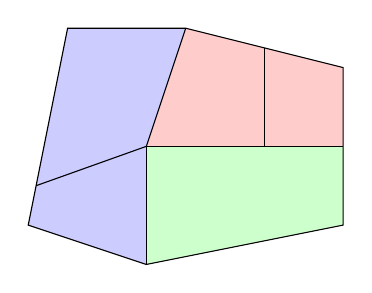
\begin{tikzpicture}[scale=0.5]
      \fill [red!20] (3, 3) -- (8, 3) -- (8, 5) -- (4, 6) -- cycle;
      \fill [green!20] (3, 0) -- (8, 1) -- (8, 3) -- (3, 3) -- cycle;
      \fill [blue!20] (0, 1) -- (3, 0) -- (3, 3) -- (4, 6) -- (1, 6) -- cycle;

      % Polygon
      \draw (3, 0) -- (8, 1) -- (8, 5) -- (4, 6) -- (1, 6) -- (0, 1) -- cycle;
      \draw (0.2, 2) -- (3, 3);
      \draw (3, 0) -- (3, 3);
      \draw (3, 3) -- (8, 3);
      \draw (6, 5.5) -- (6, 3);
      \draw (3, 3) -- (4, 6);
    \end{tikzpicture}
    \caption{Decoupage de l'espace aerien}
  \end{figure}
\end{frame}
\begin{frame}{Contexte}
  lien avec workload (written?)
  tikz secteurs valides et non \(\rightarrow\) partition
  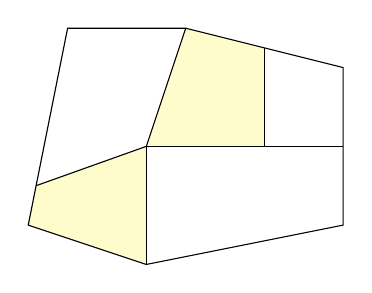
\begin{tikzpicture}[scale=0.5]
    \fill [yellow!20] (0, 1) -- (0.2, 2) -- (3, 3) -- (3, 0) -- cycle;
    \fill [yellow!20] (3, 3) -- (6, 3) -- (6, 5.5) -- (4, 6) -- cycle;

    % Polygon
    \draw (3, 0) -- (8, 1) -- (8, 5) -- (4, 6) -- (1, 6) -- (0, 1) -- cycle;
    \draw (0.2, 2) -- (3, 3);
    \draw (3, 0) -- (3, 3);
    \draw (3, 3) -- (8, 3);
    \draw (6, 5.5) -- (6, 3);
    \draw (3, 3) -- (4, 6);
  \end{tikzpicture}
  \pause{}
  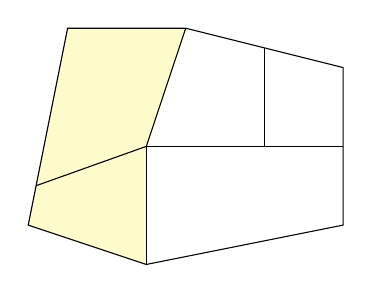
\begin{tikzpicture}[scale=0.5]
    \fill [yellow!20] (0, 1) -- (3, 0) -- (3, 3) -- (4, 6) -- (1, 6) -- cycle;

    % Polygon
    \draw (3, 0) -- (8, 1) -- (8, 5) -- (4, 6) -- (1, 6) -- (0, 1) -- cycle;
    \draw (0.2, 2) -- (3, 3);
    \draw (3, 0) -- (3, 3);
    \draw (3, 3) -- (8, 3);
    \draw (6, 5.5) -- (6, 3);
    \draw (3, 3) -- (4, 6);
  \end{tikzpicture}

\end{frame}
\begin{frame}{Transitions}
  \begin{block}{Notion de temps}
    succession de partitions
  \end{block}
  \begin{block}{Transitions}
    contraintes, \dots
  \end{block}
\end{frame}

\subsection{Modelisation de la charge de travail}
\begin{frame}{Modelisation de la charge de travail}
  \begin{block}
    {Classes}
    Quantification difficile \(\rightarrow\) classification: under, normal,
    over load
  \end{block}
  \begin{block}
    {Modele de classification}
    Simple (\# d'avions \emph{par secteur}), determinant directement la
    classe (seuils fixes) klein tikz schema
    \begin{figure}
      \subfloat[Traffic complexe]{%
        \begin{tikzpicture}[scale=0.3]
          \node [aircraft top, fill=black, scale=4] at (2, 2) {};
          \node [aircraft top, fill=black, scale=4, rotate=30] at (3, 2) {};
          % Polygon
          \draw (3, 0) -- (8, 1) -- (8, 5) -- (4, 6) -- (1, 6) -- (0, 1) --
            cycle;
          \draw (0.2, 2) -- (3, 3);
          \draw (3, 0) -- (3, 3);
          \draw (3, 3) -- (8, 3);
          \draw (6, 5.5) -- (6, 3);
          \draw (3, 3) -- (4, 6);
        \end{tikzpicture}
      }\qquad
      \subfloat[Traffic simple]{%
        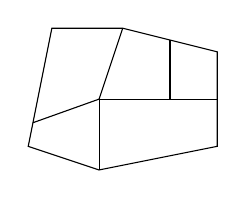
\begin{tikzpicture}[scale=0.3]

          % Polygon
          \draw (3, 0) -- (8, 1) -- (8, 5) -- (4, 6) -- (1, 6) -- (0, 1) --
            cycle;
          \draw (0.2, 2) -- (3, 3);
          \draw (3, 0) -- (3, 3);
          \draw (3, 3) -- (8, 3);
          \draw (6, 5.5) -- (6, 3);
          \draw (3, 3) -- (4, 6);
        \end{tikzpicture}
      }
    \end{figure}
  \end{block}
\end{frame}


\subsection{Construction de la fonction objectif}
\begin{frame}{Cout de partition}
  \begin{block}{Agglomeration des classifications}
    Secteur \(\to\) partition\\
    En trois couts intermediaires de sous, sur ou normale charge (\(c_+, c_-,
    c_=\))
  \end{block}
  \begin{block}{Cout resultant}
    cout d'une partition \(P\) a un temps \(t\):
    \begin{equation}
      C(P,t) = \alpha c_+ + \beta c_= + \gamma c_- + \lambda \vert P \vert
    \end{equation}
  \end{block}
\end{frame}
\begin{frame}[c]{Cout de transition}
  \begin{block}{Signification}
  Coordination entre controleurs
  \end{block}
  \begin{equation}
    C_\text{tr}(P_1, P_2) =
    \begin{cases}
      0 & \text{si\;} P_1 = P_2\\
      \theta & \text{sinon}
    \end{cases}
  \end{equation}
\end{frame}
\begin{frame}[c]{Fonction objectif}
  Cout d'une sequence de partitions \(\pi = [P_0, \dots, P_n]\),
  \begin{equation}
    f(\pi) = C(P_0, t_0) + \sum_{i=1}^n \left[
      C(P_i, t_i) + C_\text{tr}(P_{i-1}, P_i)
    \right]
  \end{equation}
\end{frame}

\section{Methode de resolution}
\subsection{Principe}
\begin{frame}[c]{Principe}
  \begin{block}{Recherche arborescente de Monte Carlo}
    \begin{itemize}
      \item Structure arborescente
      \item Parcours en profondeur
      \item Evaluation des n\oe{}uds par simulations de Monte Carlo
      \item Recherche d'un chemin
    \end{itemize}
  \end{block}
  \begin{block}{Arbres}
    \begin{itemize}
      \item Arbre de recherche
      \item Arbre de modele
    \end{itemize}
  \end{block}
\end{frame}

\subsection{Utilisation du modele}
\begin{frame}[c]{Utilisation du modele}
  \begin{block}{N\oe{}ud}
    A chaque n\oe{}ud est associe une partition
  \end{block}
  \begin{block}{Production}
    \begin{figure}
    \begin{center}
      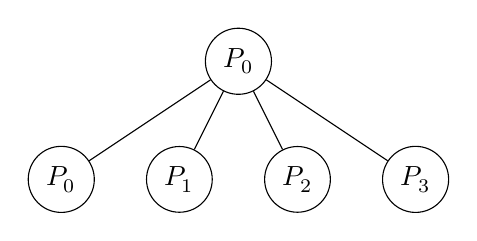
\begin{tikzpicture}[scale=1]
      \node [circle, draw] {\(P_0\)}
        child {node [circle, draw] {\(P_0\)}}
        child {node [circle, draw] {\(P_1\)}}
        child {node [circle, draw] {\(P_2\)}}
        child {node [circle, draw] {\(P_3\)}};
    \end{tikzpicture}
    \end{center}
    \caption{Representation des transitions, \(P_1, P_2\) et \(P_3\)
    atteignables depuis \(P_0\)}
    \label{fig:}
    \end{figure}

  \end{block}
\end{frame}

\subsection{Phases}
\begin{frame}[t]{Selection et expansion}
  \begin{columns}
    \begin{column}{0.5\textwidth}
      \begin{block}{Selection}
        Choix d'un chemin dans l'arbre de recherche.
        \begin{figure}
          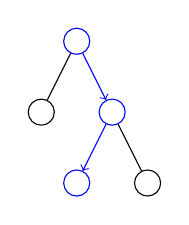
\begin{tikzpicture}[scale=0.6]
            \node [circle, draw, blue] {}
              child {node [circle, draw] {}}
              child[->, blue] {%
                node [circle, draw] {}
                child[->] {node [circle, draw] {}}
                child[-, black] {node [circle, draw] {}}
              };
          \end{tikzpicture}
          \caption{Sélection d'un chemin}
        \end{figure}
      \end{block}
    \end{column}
    \begin{column}{0.5\textwidth}
      \begin{block}{Expansion}
        Ajout d'un n\oe{}ud a l'arbre de recherche.
        \begin{figure}
          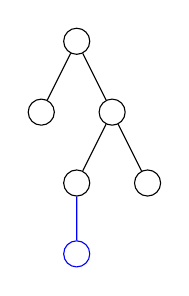
\begin{tikzpicture}[scale=0.6]
            \node [circle, draw] {}
              child {node [circle, draw] {}}
              child {%
                node [circle, draw] {}
                child {%
                  node [circle, draw] {}
                  child [circle, draw, blue] {node [circle, draw] {}}
                }
                child {node [circle, draw] {}}
              };
          \end{tikzpicture}
          \caption{Expansion}
        \end{figure}
      \end{block}
    \end{column}
  \end{columns}
\end{frame}
\begin{frame}[t]{Simulation et sauvegarde}
  \begin{columns}
    \begin{column}{0.5\textwidth}
      \begin{block}{Simulation}
        Évaluation d'un n\oe{}ud ajoute.
        \begin{figure}
          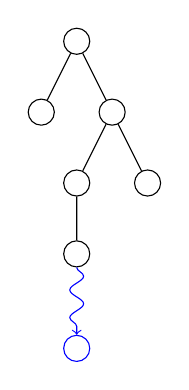
\begin{tikzpicture}[scale=0.6]
            \node [circle, draw] {}
              child {node [circle, draw] {}}
              child {%
                node [circle, draw] {}
                child {%
                  node [circle, draw] {}
                  child [circle, draw] {node (l) [circle, draw] {}}
                }
                child {node [circle, draw] {}}
              };

            \draw[blue] (l) ++(0, -2) node(s) [circle, draw] {};
            \draw[->, blue, decorate, decoration={snake}] (l) -- (s);
          \end{tikzpicture}
        \caption{Simulation}
        \end{figure}
      \end{block}
    \end{column}
    \begin{column}{0.5\textwidth}
      \begin{block}{Sauvegarde}
        Mise a jour de l'ensemble de l'arbre de recherche.
      \end{block}
      \begin{figure}
        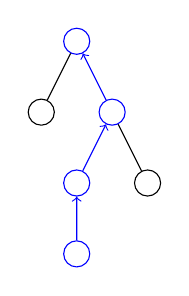
\begin{tikzpicture}[scale=0.6]
          \node [circle, draw, blue] {}
            child {node [circle, draw] {}}
            child[<-, blue] {%
              node [circle, draw] {}
              child {%
                node [circle, draw] {}
                child [circle, draw] {node [circle, draw] {}}
              }
              child[-, black] {node [circle, draw] {}}
            };
        \end{tikzpicture}
        \caption{}
      \end{figure}
      
    \end{column}
  \end{columns}
\end{frame}

\subsection{Construction de la solution}
\begin{frame}[c]{Construction de la solution}
  \begin{block}{Selection v.\ choix final}
  \end{block}
  \begin{block}{Construction iterative de chemin}
    \begin{itemize}
      \item Une passe Monte Carlo permet de choisir un noeud,
      \item appels recursifs pour construire un chemin.
    \end{itemize}
  \end{block}
\end{frame}

\subsection{A\(^*\)}
\begin{frame}[c]{A\(^*\)}
  \begin{block}{Principe}
    \begin{itemize}
      \item Methode exacte
      \item Parcours en profondeur
      \item Utilisation d'une heuristique
    \end{itemize}
  \end{block}
  \begin{block}{Heuristique}
    \begin{itemize}
      \item \(h(u)\): cout du chemin allant de \(u\) jusqu'a une feuille,
      \item utilisations des partitions optimales, même si non atteignables
    \end{itemize}
  \end{block}
\end{frame}

\section{Résultats}

\section*{Conclusion}
\end{document}
